\documentclass[tikz,border=8pt]{standalone}
\usepackage{amsmath}
\usepackage{amssymb}
\usetikzlibrary{arrows.meta,calc,positioning}

\definecolor{basisblue}{HTML}{2F6F9F}
\definecolor{basisgreen}{HTML}{5F7F55}
\definecolor{basisgold}{HTML}{A66F00}
\definecolor{textgray}{HTML}{2F3437}
\definecolor{linegray}{HTML}{AEB7BC}
\definecolor{softgray}{HTML}{F5F7F8}

\begin{document}
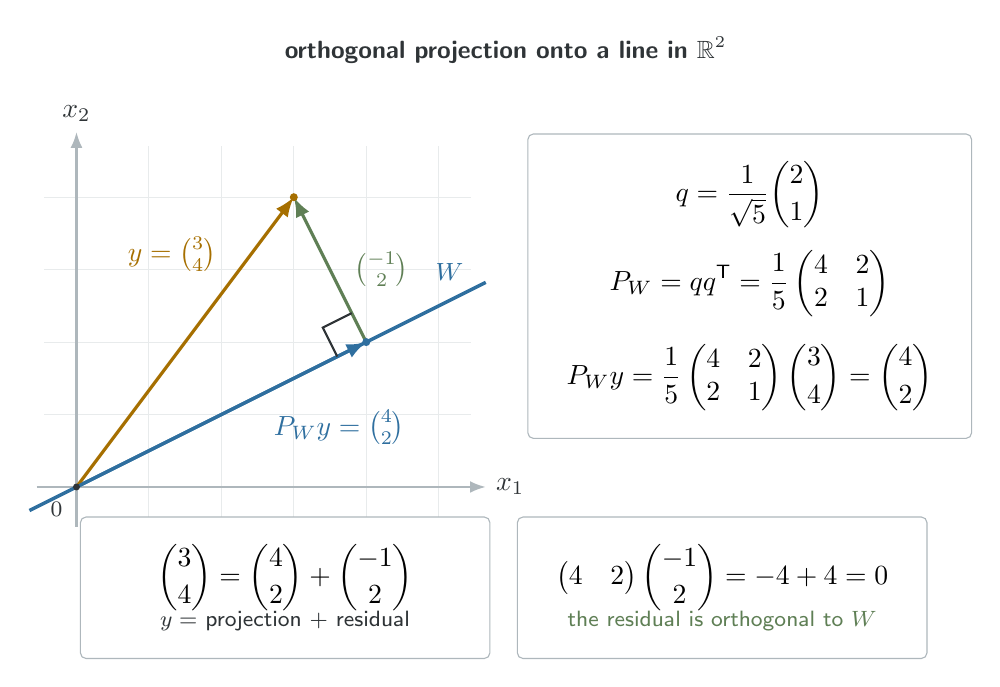
\begin{tikzpicture}[
  font=\sffamily,
  >=Latex,
  vector/.style={-{Latex[length=2.5mm]}, line width=1.15pt},
  axis/.style={-{Latex[length=2mm]}, draw=linegray, line width=0.75pt},
  guide/.style={draw=linegray, dashed, line width=0.65pt},
  stage/.style={
    draw=linegray,
    fill=white,
    rounded corners=2pt,
    inner xsep=14pt,
    inner ysep=10pt,
    align=center
  },
  label/.style={font=\sffamily\bfseries\small, text=textgray},
  smallnote/.style={font=\sffamily\small, text=textgray, align=center},
  mathnote/.style={font=\sffamily\footnotesize, text=textgray, align=center}
]

\node[label] at (5.45,5.55) {orthogonal projection onto a line in $\mathbb R^2$};

% Coordinate picture for the exact vectors in the example.
\begin{scope}[x=0.92cm,y=0.92cm]
  \draw[draw=linegray!28, step=1] (-0.45,-0.45) grid (5.45,4.70);
  \draw[axis] (-0.55,0) -- (5.65,0) node[right, text=textgray] {$x_1$};
  \draw[axis] (0,-0.55) -- (0,4.90) node[above, text=textgray] {$x_2$};

  % W has direction (2,1), hence slope 1/2.
  \draw[draw=basisblue, line width=1.25pt]
    (-0.65,-0.325) -- (5.65,2.825);
  \node[smallnote, text=basisblue, anchor=south]
    at (5.15,2.72) {$W$};

  % y, its projection, and the residual drawn head-to-tail.
  \draw[vector, draw=basisgold] (0,0) -- (3,4)
    node[pos=0.70, above left=1pt, text=basisgold] {$y=\binom{3}{4}$};
  \draw[vector, draw=basisblue] (0,0) -- (4,2)
    node[pos=0.63, below right=2pt, text=basisblue] {$P_Wy=\binom{4}{2}$};
  \draw[vector, draw=basisgreen] (4,2) -- (3,4)
    node[midway, right=5pt, text=basisgreen] {$\binom{-1}{2}$};

  \fill[textgray] (0,0) circle (1.25pt);
  \fill[basisblue] (4,2) circle (1.45pt);
  \fill[basisgold] (3,4) circle (1.45pt);

  % Right-angle marker: (-2,-1) is perpendicular to (-1,2).
  \draw[draw=textgray, line width=0.75pt]
    (3.60,1.80) -- (3.40,2.20) -- (3.80,2.40);

  \node[mathnote, anchor=north east] at (-0.06,-0.08) {$0$};
\end{scope}

% The numerical projection calculation.
\node[stage, minimum width=5.0cm] at (8.55,2.55) {
  $\displaystyle q=\frac{1}{\sqrt5}\binom{2}{1}$\\[7pt]
  $\displaystyle P_W=qq^{\mathsf T}
    =\frac15\begin{pmatrix}4&2\\2&1\end{pmatrix}$\\[9pt]
  $\displaystyle P_Wy
    =\frac15\begin{pmatrix}4&2\\2&1\end{pmatrix}\binom34
    =\binom42$
};

% Decomposition and orthogonality checks.
\node[stage, minimum width=5.20cm] at (2.65,-1.28)
  {$\displaystyle \binom34=\binom42+\binom{-1}{2}$\\[-1pt]
   \textcolor{textgray}{\footnotesize $y=$ projection $+$ residual}};

\node[stage, minimum width=5.20cm] at (8.20,-1.28)
  {$\displaystyle \begin{pmatrix}4&2\end{pmatrix}\binom{-1}{2}=-4+4=0$\\[-1pt]
   \textcolor{basisgreen}{\footnotesize the residual is orthogonal to $W$}};

\end{tikzpicture}
\end{document}
